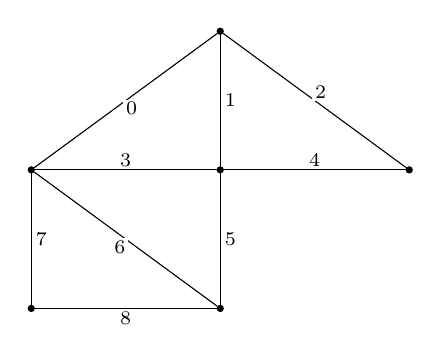
\begin{tikzpicture}[x=0.8cm,y=0.8cm,baseline=(current bounding box.center)]
  \tikzset{graphvertex/.style={circle,fill=black,draw=black,inner sep=0pt,minimum size=2.2pt}}
  \tikzset{graphedge/.style={draw=black,line width=0.4pt}}
  \tikzset{edgelabel/.style={font=\scriptsize,inner sep=1pt,fill=white,text=black}}
  \node[graphvertex] (v0) at (0.000,2.200) {};
  \node[graphvertex] (v1) at (-3.000,0.000) {};
  \node[graphvertex] (v2) at (0.000,0.000) {};
  \node[graphvertex] (v3) at (3.000,0.000) {};
  \node[graphvertex] (v4) at (0.000,-2.200) {};
  \node[graphvertex] (v5) at (-3.000,-2.200) {};
  \draw[graphedge] (v0) -- (v1);
  \node[edgelabel] at (-1.405,0.971) {0};
  \draw[graphedge] (v0) -- (v2);
  \node[edgelabel] at (0.160,1.100) {1};
  \draw[graphedge] (v0) -- (v3);
  \node[edgelabel] at (1.595,1.229) {2};
  \draw[graphedge] (v1) -- (v2);
  \node[edgelabel] at (-1.500,0.160) {3};
  \draw[graphedge] (v2) -- (v3);
  \node[edgelabel] at (1.500,0.160) {4};
  \draw[graphedge] (v2) -- (v4);
  \node[edgelabel] at (0.160,-1.100) {5};
  \draw[graphedge] (v4) -- (v1);
  \node[edgelabel] at (-1.595,-1.229) {6};
  \draw[graphedge] (v1) -- (v5);
  \node[edgelabel] at (-2.840,-1.100) {7};
  \draw[graphedge] (v4) -- (v5);
  \node[edgelabel] at (-1.500,-2.360) {8};
\end{tikzpicture}
